
We first verify that the simulation's output matches obviously expected
results. Then, in the following section, we investigate aspects of its behavior
which are not computable analytically in order to discover important
consequences of the model.


\subsection{Agent and proto life history}

For a sensible range of parameter settings, the life history of a single
simulation run follows an expected pattern. Assuming a positive growth rate
(\textit{i.e.}, salary > metabolic rate), each agent's wealth rises unsteadily
during stage 1, until eventually the first pair of neighboring agents who each
reach the threshold form a proto-institution. Throughout stage 2, these agents
contribute all wealth in excess of the threshold to that proto, and so their
proto's balance rises unsteadily while their personal wealth remains at the
constant threshold. Meanwhile, the other agents also reach the threshold at
various points in time, and also form or join protos, until every non-isolate
(that is, every node with at least one neighbor) is a member of a proto. Stage
3 (the starvation period) then commences, with isolates drawing on a greater
personal wealth than the non-isolates. When an isolate reaches zero wealth, it
dies; when a non-isolate reaches zero, it draws from its (shared) proto balance
until that too, reaches zero, and it dies.

\begin{figure}[ht]
\centering
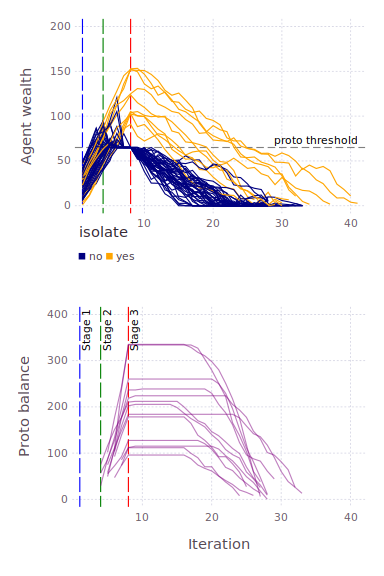
\includegraphics[width=\columnwidth]{figures/sampleLifeHistory.png}
\caption{A single run of the simulation, with $\lambda$=2. Each of 50 nodes is
given an initial wealth of $\sim\mathcal{U}(0,50)$ units, a regular income
distributed as $\sim\mathcal{N}(20,5)$, a metabolic rate of 5, and a proto
threshold of 65.} \label{fig:singleRun}
\end{figure}

This history can be seen in Figure~\ref{fig:singleRun}. The top plot depicts
agent wealth at every iteration, and the bottom plot shows the balances of the
protos at the same points in time. (No protos exist until stage 2, by
definition.) Note that the isolates (orange lines) never form protos, and
therefore begin the starvation stage with a higher personal wealth to draw
from.


\begin{figure}[ht]
\centering
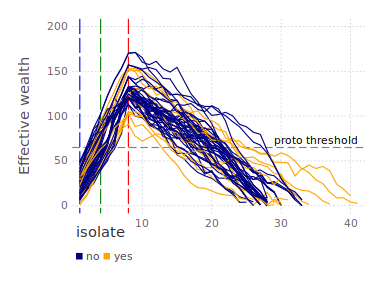
\includegraphics[width=\columnwidth]{figures/sampleEffectiveHistory.png}
\caption{The same simulation run as Figure~\ref{fig:singleRun}, but this time
depicting each agent's \textit{effective} wealth (its personal wealth plus its
share of its proto's wealth, if any).}
\label{fig:effectiveWealthSingleRun}
\end{figure}

Figure~\ref{fig:effectiveWealthSingleRun} shows the same information in another
way: instead of plotting each agent's \textit{personal} wealth (as in the top
plot of Figure~\ref{fig:singleRun}), we show its \textbf{effective wealth},
defined as the sum of its personal wealth and its ``share'' of its proto's
wealth (if any). After all, contributions that a proto's members make to its
balance are available to those members in times of need; therefore, a fair
comparison between isolates and non-isolates should take this into account.
From the figure, it can be seen that isolates no longer have a systematic
advantage (as they appeared to in Figure~\ref{fig:singleRun}.)

We verified that changes to basic parameters all have the expected effect:
lowering the initial wealth delays the onset of stage 2; a higher $\sigma^2$
for the income distribution makes the lines less jagged; a higher metabolic
rate hastens extinction; \textit{etc.}

\subsection{Gini coefficient history}

% Will's paragraph goes here, references Figure~\ref{fig:giniHistory}.

\begin{figure}[hb]
\centering
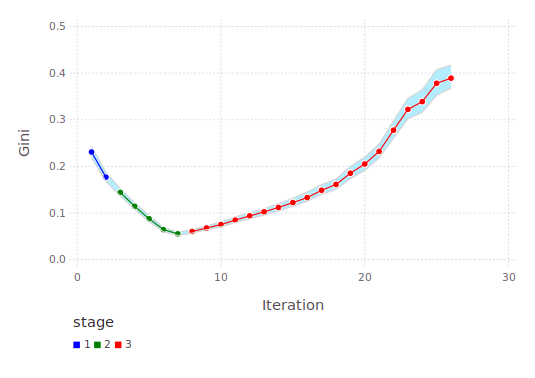
\includegraphics[width=\columnwidth]{figures/giniHistory.png}
\caption{The simulated society's wealth inequality over time. (The same
simulation parameters were used as in Figures~\ref{fig:singleRun} and
\ref{fig:effectiveWealthSingleRun}, but this time with 500 agents.) The light
blue band represents a bootstrapped 95\% confidence interval.}
\label{fig:giniHistory}
\end{figure}

    The Gini coefficient of the agent population as seen in the top plot of Figure~\ref{fig:giniHistory} is influenced by two distinct dynamics: loss/accumulation of wealth and the formation/death of proto-institutions. Over the course of Stage 1 and the beginning of Stage 3, this change in agent wealth is exclusively responsible for changes in the Gini coefficient. As agents accumulate wealth over Stage 1 and 2, the size of wealth differentials shrinks relative to absolute agent wealth, leading to the declining Gini coefficient. The opposite effect occurs during Stage 3 as agent starvation leads to the relative growth of these wealth differentials. The variability in starvation rates further contributes to the increasing Gini coefficient.

    In addition, as indicated in the bottom plot, the proto formation and proto death also influence the Gini coefficient during Stage 2 and the end of Stage 3, respectively. As expected, the formation of protos during Stage 2 contributes to declining Gini coefficient as the constituent agents of each proto have equivalent wealth values and represent coalitions of perfect economic equality. Accordingly, the death of protos, beginning around Iteration 20, contributes to increase the Gini coefficient by removing the protos' effect on the system's inequality. 

    (Note: As the population size decreases over the starvation period, the Gini coefficient becomes increasingly unstable and susceptible to small fluctuations in agent wealth; hence the erratic nature of the red line at the extreme right of Figure~\ref{fig:giniHistory}.)

% vim:textwidth=99999
